\section{Interfaccia Utente}
Per quanto riguarda l'interfaccia utente, si voleva avere una visualizzazione chiara
e semplice dei propri meeting in programma, per questo è stato scelto un calendario.
\\
Più precisamente si è deciso di utilizzare \textit{FullCalendar} \cite{FullCalendarSite},
una famosa libreria Javascript open source che si integra perfettamente con React.

\begin{figure}[H]
    \centering
    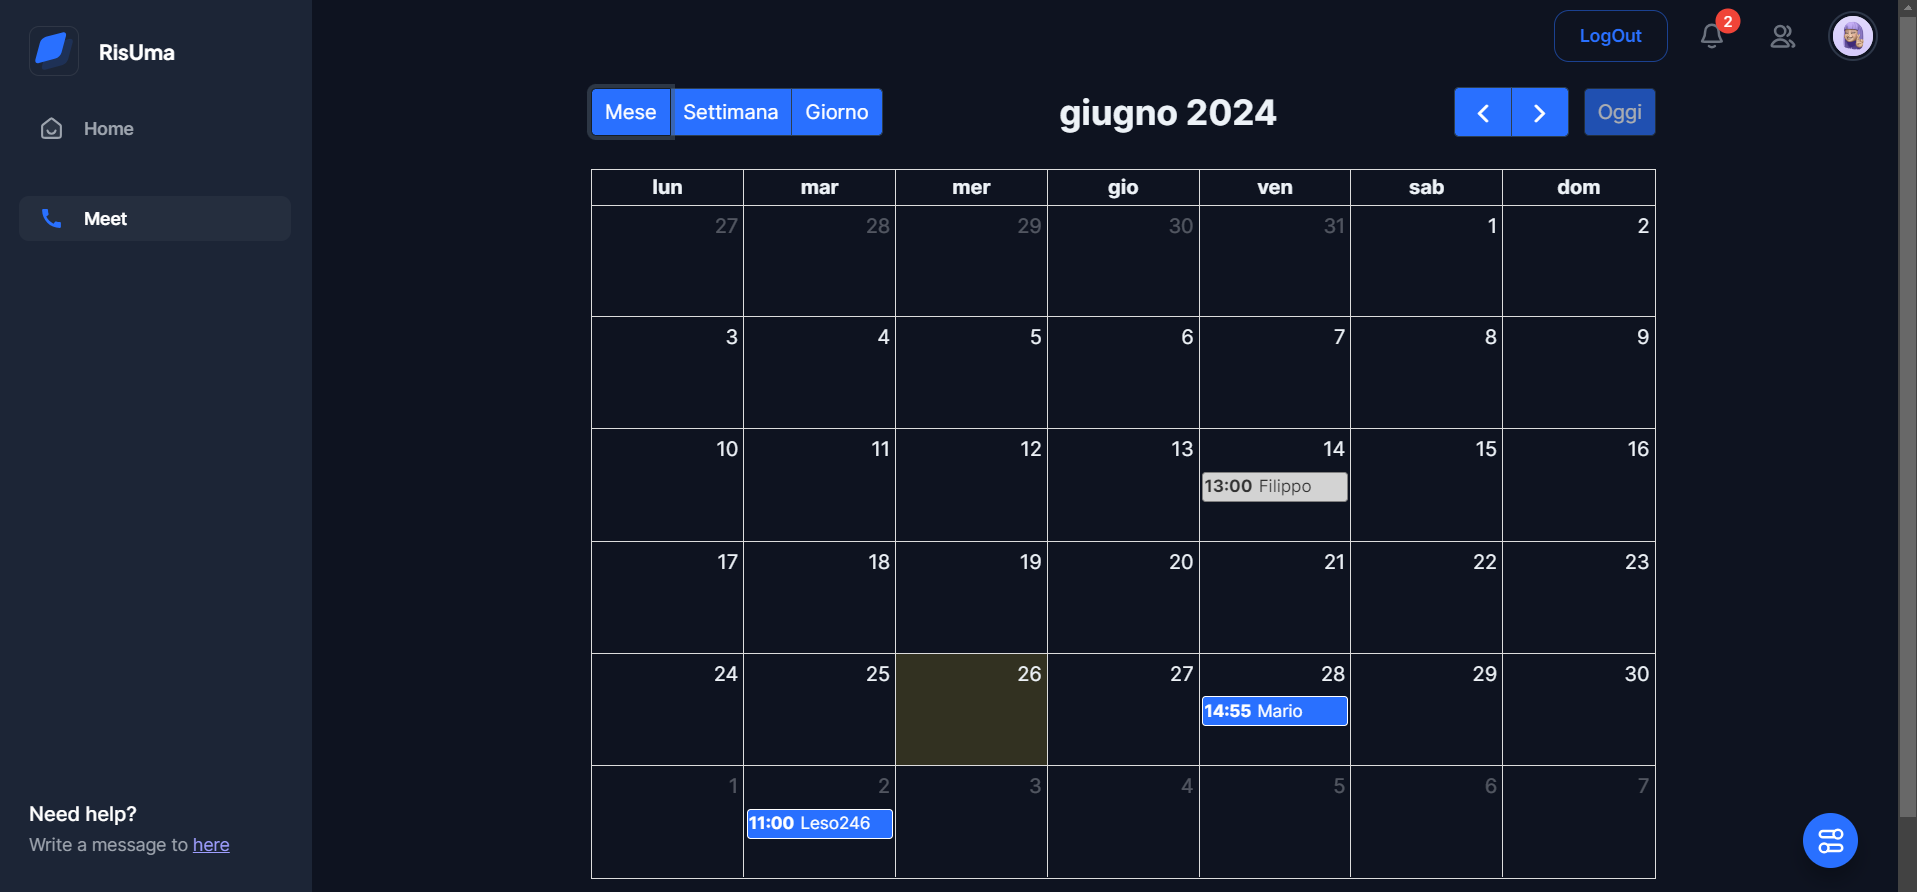
\includegraphics[width=1\textwidth]{../screenshot/visualizzazione claendario/tema scuro calendario.png}
    \caption{Example image}
    \label{img:visualizzazione_calendario_interfaccia_utente}
\end{figure}

